\section*{Threat Evaluation}
\addcontentsline{toc}{section}{Threat Evaluation}

Following the identification of the supporting asset, a set of threats and related vulnerabilities were described. 

As shown in figure \ref{fig:threatsEval}, the threats with the highest impacts are the ones tied to the private network and the virtual desktop infrastructure. In particular, those threats are unauthorized wired connections and hyperjacking\cite{online:hyperjacking}. 

These threats were chosen assuming poor access control on the routing equipment of the network and by searching for disrupting incidents for hypervisors. 

Another class belongs to the physical realm. More specifically, the threats tied to the physical access to the server rooms and the natural incidents to which the appliances can be exposed were taken into consideration. As can be seen in the table, the impact of these threats is high and cannot be left untreated.

Finally, only the two threats tied to the \texttt{GSB LAN gateway} were found to have attenuating circumstances. This is because we are considering the gateway of a single municipality, so the incidents will be limited to that GSB.

\begin{figure}[h!]
    \centering
    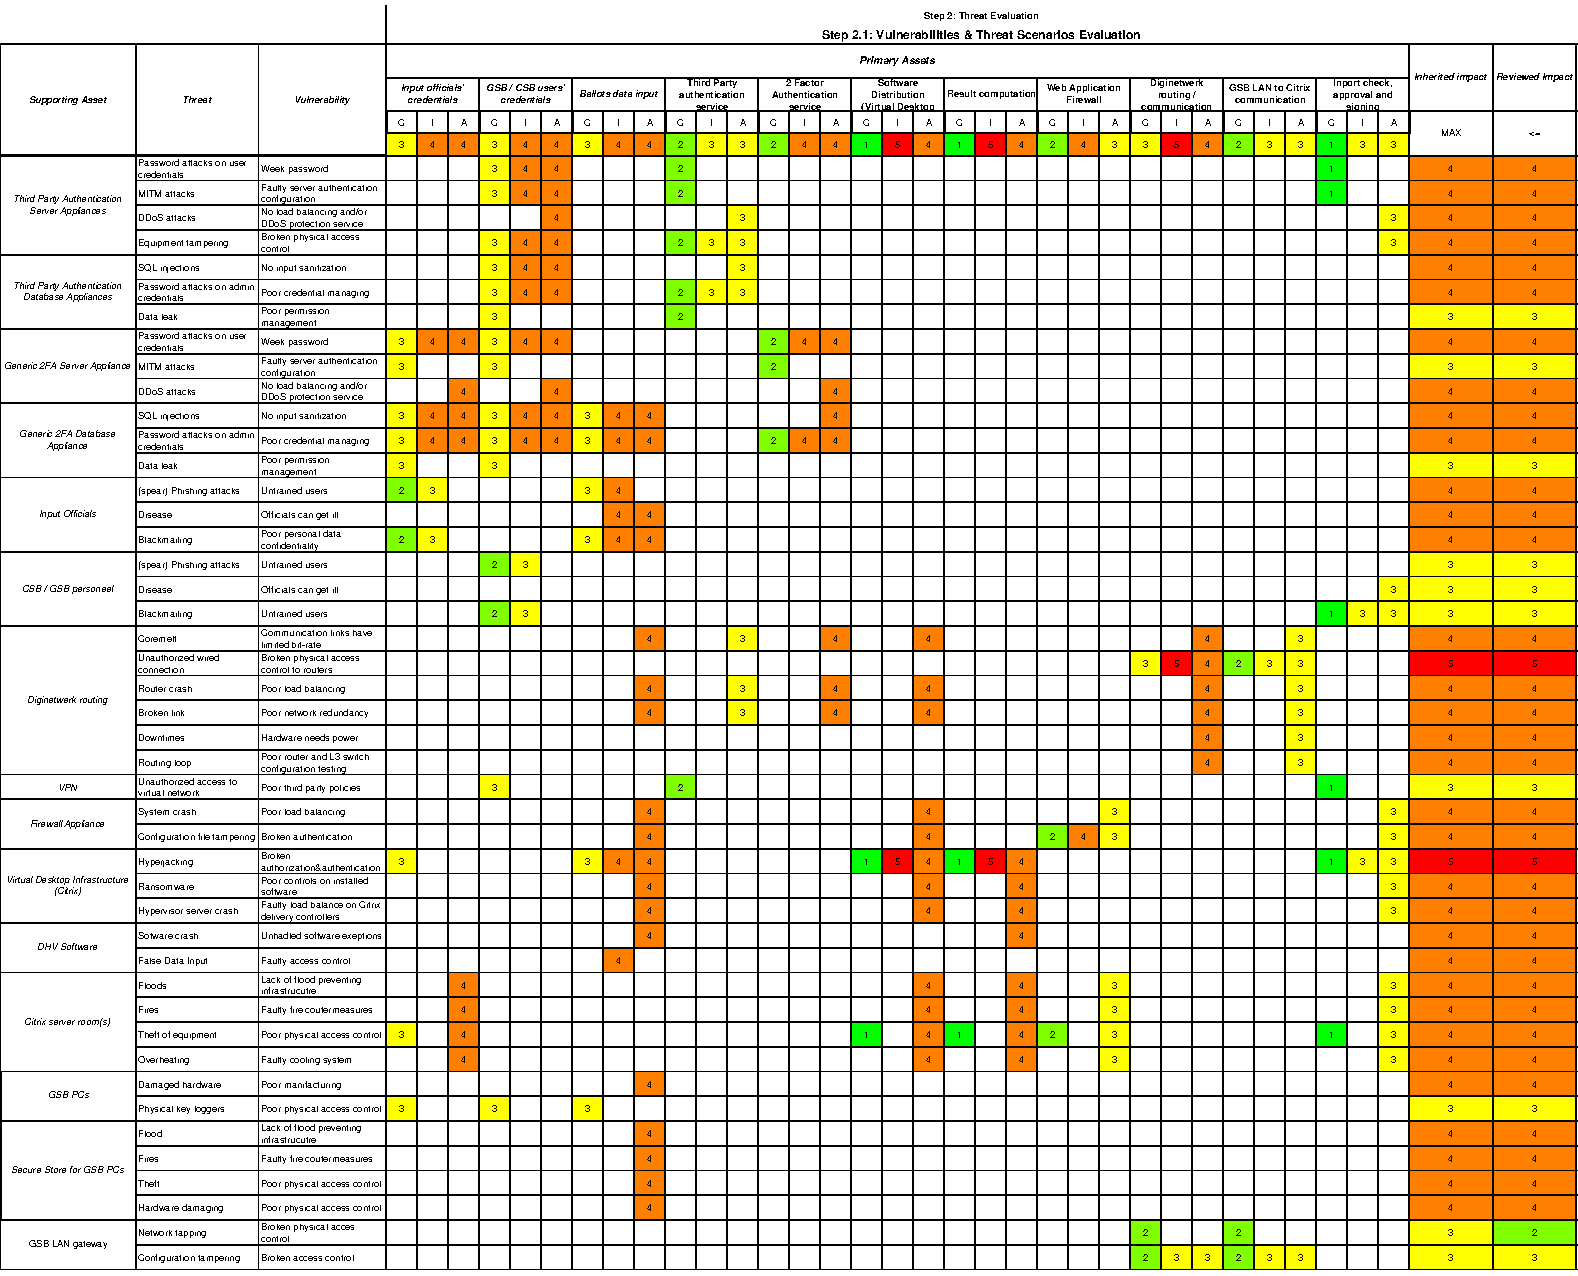
\includegraphics[keepaspectratio,width=1\textwidth]{03-risk-analysis/003-TE/img/threatEval.pdf}
    \caption{Threat evaluation table}
    \label{fig:threatsEval}
\end{figure}

\newpage

Figure \ref{fig:likelihood} shows how likely it is for an incident tied to a threat to happen. For accidental incidents and natural disasters, only the overall score is assigned.

As can be seen in the table, the majority of the threats with higher impacts like Coremelt are mitigated by their low likelihood. Unfortunately, threats like hyperjacking, equipment theft, and tampering still retain a high likelihood score.

Also, historical events were taken into consideration. In particular, since this system is deployed in the Netherlands, data about flooding was researched\cite{online:flooding}.

Note that justifications for the likelihood table can be found in the excel file.

\begin{figure}[]
    \centering
    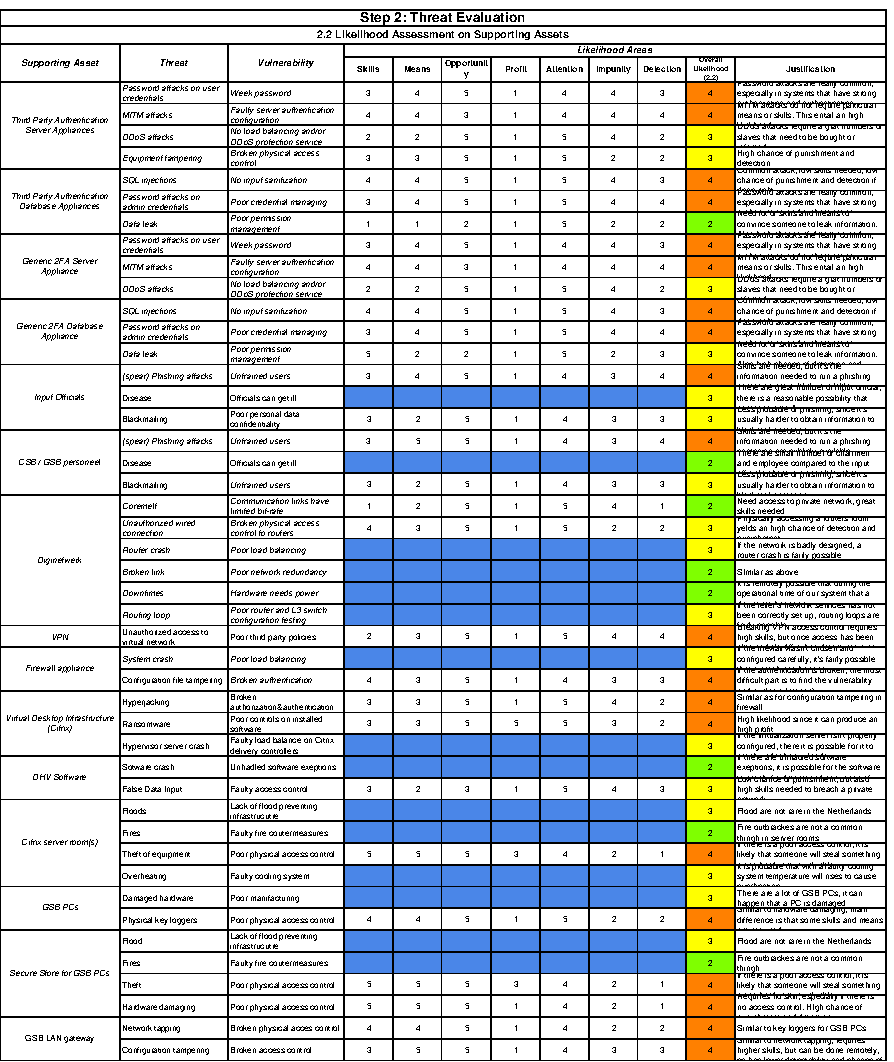
\includegraphics[keepaspectratio,width=1\textwidth]{03-risk-analysis/003-TE/img/likelihood.pdf}
    \caption{Threat likelihood table}
    \label{fig:likelihood}
\end{figure}